We apply a data-driven method to estimate the $H \to \WW$ jet counting 
efficiency and its systematic uncertainties in data. 
In this method, the $H \to \WW$ jet counting efficiency in data $\epsilon_{H \to \WW}$
is estimated to be the value obtained from simulation multiplied by a data to simulation
scale factor from \dyll~events such that,

$$\epsilon_{H \to \WW} = \epsilon_{\Z}^{data} (\frac{\epsilon_{H \to \WW}}{\epsilon_{\Z}})^{MC}.$$

The uncertainty in $\epsilon_{H \to \WW}$ can be factorized into the 
$\Z$ efficiency uncertainty in data and the $H \to \WW/\Z$ efficiency ratio 
uncertainty in simulation. 
The former is dominated by the statistical uncertainty, while 
theoretical uncertainties due to higher order corrections contribute most 
to the $H \to \WW/\Z$ efficiency ratio uncertainties. 

The jet multiplicity distribution for $\dyll$ events in data is compared with the 
values obtained from Powheg simulation as shown in Figure~\ref{fig:njets_dyll}. 
The data to simulation correction factor is close to unity for the zero-jet and 1-jet bins, 
while we observe some disagreement for events with at least two reconstructd jets. 
This is not surprising since Powheg is an NLO generator, and 
only expected to produce an accurate description for events 
containing up to one jet. For instance, the comparison between data and Madgraph 
simulation, which accounts for leading order diagrams containing up to four additional
partons, gives much better agreement in the 2-jet bin. 

The jet spectrum is correctly simulated for the Higgs signal since we
reweight the Higgs $\pt$ spectrum is to the NNLO+NNLL differential calculation. 
As a result no correction is applied on top of the jet spectrum simulated for the Higgs signal, 
reweighted in the Higgs $\pt$ spectrum to the NNLO+NNLL differential calculation.

\begin{figure}[!htbp]
\begin{center}
   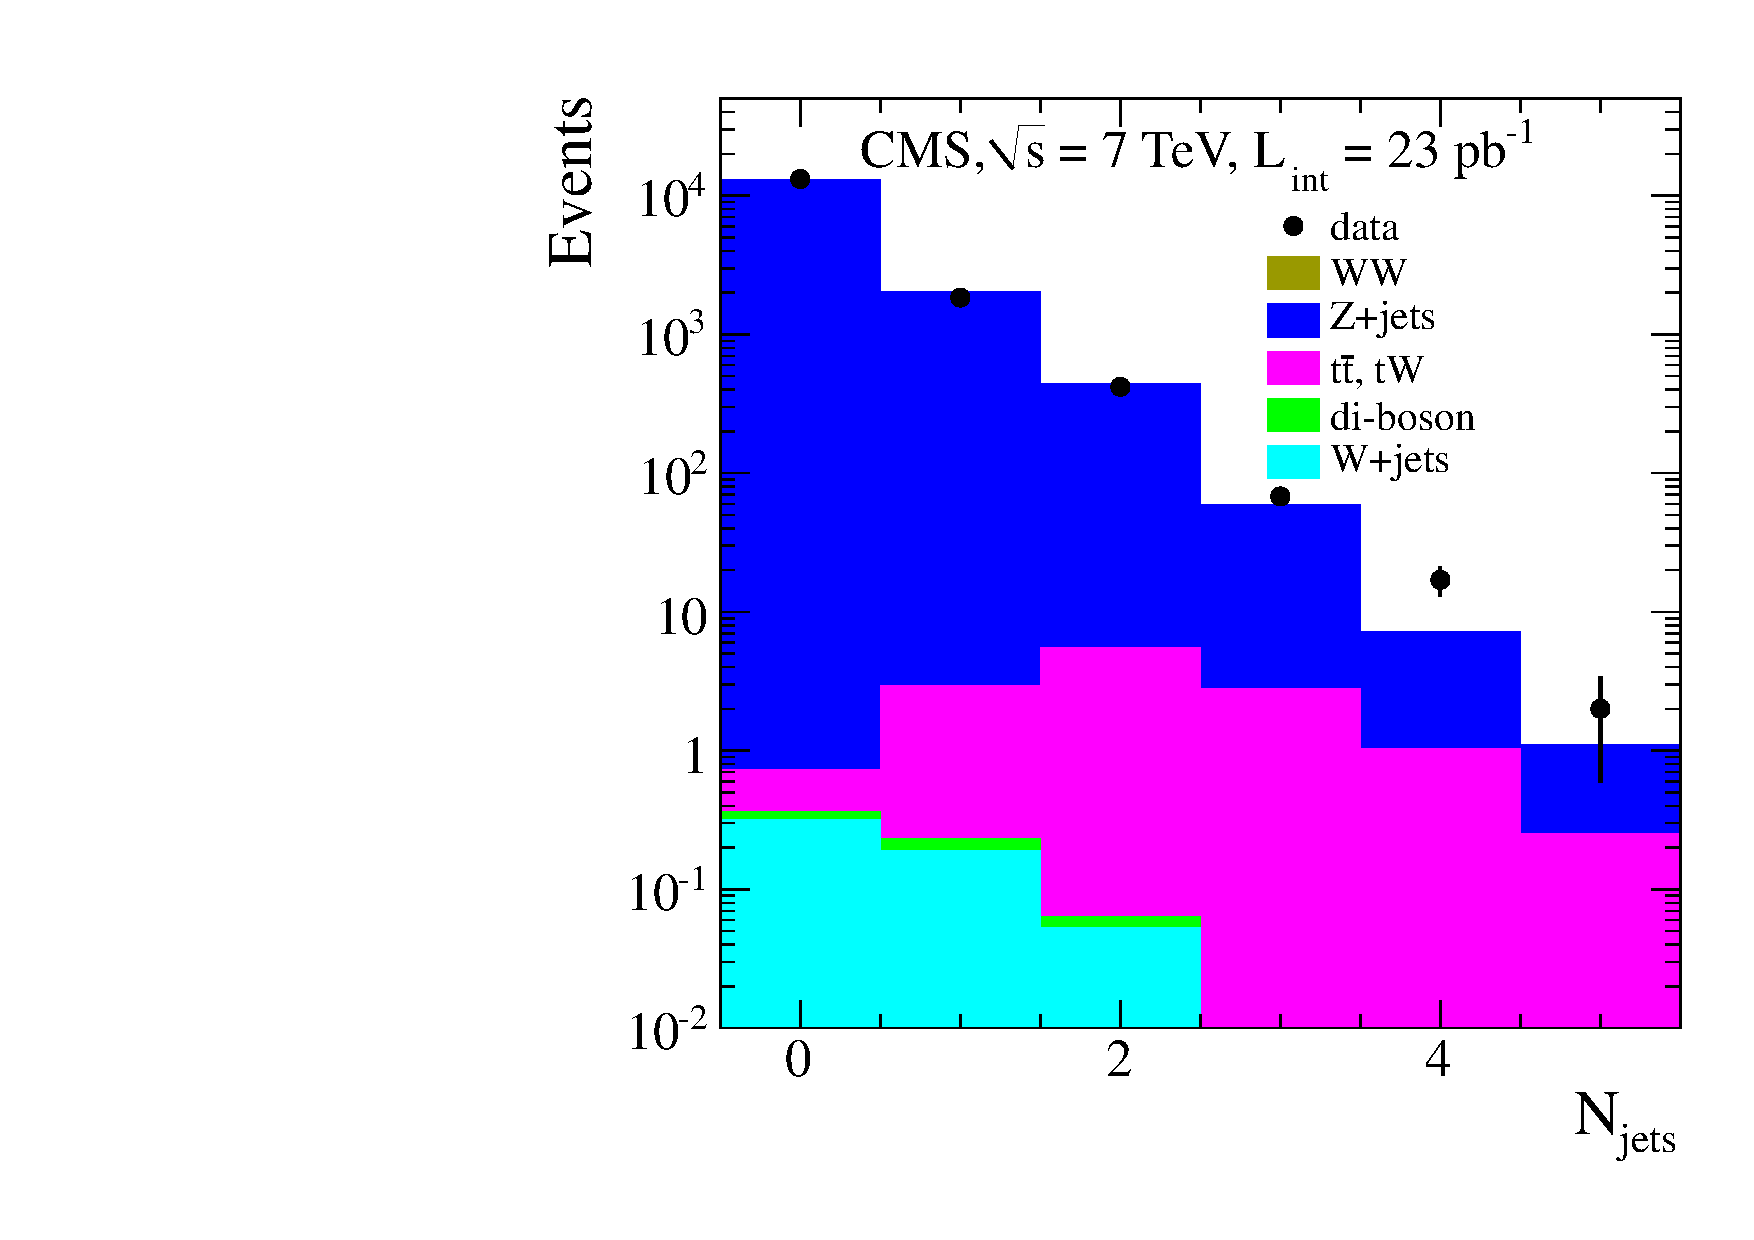
\includegraphics[width=0.60\textwidth]{figures/njets_dyll.pdf}
   \caption{Jet multiplicity distribution for $\dyll$ events.}
   \label{fig:njets_dyll}
\end{center}
\end{figure}
